% \begin{tikzpicture}[text centered]
	\draw[legende] (-3.25,10) rectangle (3.25,-2.5);
	\node[text width=5cm] at (0,9.3) {\strong{création de séquences dégradées par classe de contenu}};
	\node at (0,7) {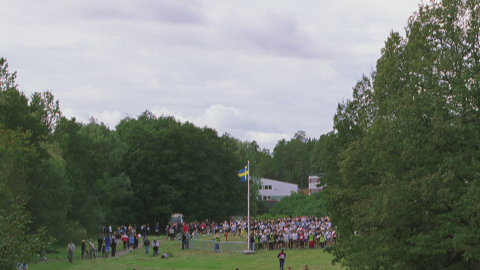
\includegraphics[width=6cm]{img/chap3/aboveMarathon}};
	\draw (-3,8) -- (-1.5,7.3) -- (1.1,7.3) -- (2.2,8.7);
	\node[legende,font=\small] at (-0.5,8) {zone uniforme};
	\node at (0,3.5) {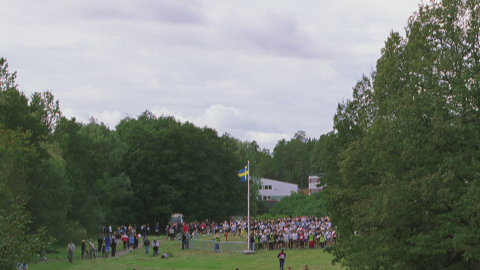
\includegraphics[width=6cm]{img/chap3/aboveMarathon}};
	\draw (-2.5,1.8) -- (-1.6,2.5) -- (1.2,2.5) -- (1.2,1.8);
	\node[legende,font=\small] at (-0.5,2.15) {textures fines};
	\node at (0,0) {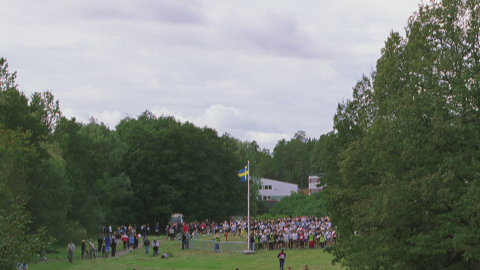
\includegraphics[width=6cm]{img/chap3/aboveMarathon}};
	\draw (-3,1) -- (-1.5,0.3) -- (1.1,0.3) -- (2.2,1.7);
	\draw (-2.5,-1.7) -- (-1.6,-1) -- (1.2,-1) -- (1.2,-1.7);
	\node[legende,font=\small] at (0,-0.5) {textures fortes et structurées};
	\node at (0,-2.1) {\dots};

	\node[action,text width=2cm] (node) at (6,7) {tests SAMVIQ};
	\draw[fleche] (3.25,7) -- (node);
	\draw[fleche] (node) -- (8,7);

	\foreach \x in {6.5,6,5.5,5}
	{
			\draw[legende] (8,\x) rectangle (9.5,\x + 1.5);
			\draw[->] (8.25,\x + .25) -- (8.25,\x + 1.25) node[above=-0.1cm, font=\tiny] {gêne};
			\draw[->] (8.25,\x + .25) -- (9.25,\x + .25);
	}
	\node[above] at (9.25,5.25) {?};
	\node[text width=3.5cm] at (6.25,5.5) {une fonction de gêne par classe de contenu};

	\draw[fleche] (8.75,5) -- (8.75,3.5);
	\node at (8,4.25) {cumul ?};
	\draw[->] (7.75,1) -- (9.75,1) node[below] {$D$};
	\draw[->] (7.75,1) -- (7.75,3) node[left] {gêne};
% \end{tikzpicture}
